% !TEX root = ../notes_template.tex

\chapter{Cardiac Pump}\label{chp:cardiac_pump}
Updated on \today
\minitoc
This chapter covers the cardiac pump in its role to support circulation. Circulation is completely dependent on the pumping action of the cardiac muscle to create the pressure gradient for both systemic, and a bit less so, the pulmonary circulation. 

The relationship between circulation and cardiac muscle is similar to the relationship between movement and skeletal muscle. Concepts from skeletal muscle such as tension, excitation, regulation and energetics are applicable to cardiac muscle and are included. It is useful to compare and contrast cardiac muscle with skeletal muscle across these concepts while focusing on how the differences enable the cardiac muscle to meet the unique needs of circulation. The primary goal of this chapter is an understanding of cardiac pump in its supportive role for circulation. 

\vspace{5mm}
\begin{svgraybox}
\textbf{Objectives include:}
\begin{enumerate}
    \item Compare and contrast cardiac and skeletal muscle based on tension, excitation, regulation and energetics.
    \item Explain how the unique characteristics of cardiac muscle tension, excitation (automaticity, rhymicity, conductivity, contractility), regulation and energetics support circulation.
    \item Explain factors that influence cardiac output (including preload, afterload, intropy, chronotropy).
    \item Explain the relationship between RPP and myocardial oxygen demand.
    \item Explain cardiac circulation.
    \item Explain the cardiac cycle (to the point of drawing and explaining all aspects of Wiggers Diagram).
    \item Perform an ECG rhythm analysis including the identification of arrhythmias and myocardial circulation abnormalities.
\end{enumerate}
\end{svgraybox}

\section{Cardiac Muscle}

The role of the heart as a pump is based on it's ability to regularly provide the pressure necessary for circulation of blood through arterial vessels (both systemic arteries (which includes the cardiac circulation) and pulmonary arteries). The function of the heart as a pump depends on several characteristics of cardiac muscle:

\begin{itemize}
    
    \item Automaticity: The ability to initiate its own excitation
    \item Rhythmicity: The ability to repeat the its own excitation cycle in synchrony with regularity
    \item Excitability: The ability to respond to excitation with activation
    \item Conductivity: The ability to transmit excitations from cell to cell within the heart
    \item Contractility: The ability to generate a full contractile (shortening) cycle with each excitation
 
\end{itemize}

The next four sections parallel the chapters on skeletal muscle function of Part II: Tension, Excitation, Regulation and Energetics. They, in turn, compare and contrast cardiac and skeletal muscle in these key areas and also how the cardiac muscle and pump are thus uniquely capable of supporting circulation. As a reminder Chapter \ref{chp:circulation} on Circulation focused on circulation leaving the left ventricle and returning to the right atrium. This chapter is focused on the circulation through the heart itself as it is pumped and travels from the right atrium to the left ventricle. There are, however, two caveats. First, this chapter includes details about the cardiac circulation within the section on energetics (since cardiac muscle energetics is very dependent on the regular delivery of oxygen via blood flow). Second, this chapter does not include details on the pulmonary circulation (leaving the right ventricle and returning to the left atrium). The pulmonary circulation is covered in the next chapter on Respiration.

\subsection{Tension}

It is reasonable to use the term contraction when describing activation and active tension for the cardiac muscle because contraction (shortening) is what occurs (there is no eccentric or isometric activation of cardiac muscle). A major difference between cardiac and skeletal muscle is that cardiac muscle does not have a tendon attachment. Cardiac muscle attaches to itself to create a chamber that has a volume. When cardiac muscle contracts, it makes the chamber smaller (less volume). In skeletal muscle the length of fibers translates into the length of the entire muscle and this relationship has a functional interpretation. In cardiac muscle the length of fibers directly translates into the volume of chambers. It is the volume of these chambers that has a functional interpretation. 

The heart has four chambers that function as four pumps (right and left atria; right and left ventricles). From a muscular perspective there are two chambers, each separated into a right and a left side with a relatively thin muscular barrier between them. This is quite noticeable in conditions that result in abnormal timing of the right and left ventricle excitation. If the ventricles are not excited at the same time, off even by 50 milliseconds, the overall pump effectiveness of both ventricles is impaired (mechanical cardiac asynchrony).

\paragraph{Active Tension}

Active tension is generated in cardiac muscle with the same sliding filament model of skeletal muscle described in Chapter \ref{chp:tension} on Tension. Active tension generates tension that shortens cardiac muscle fibers and makes the cardiac chambers smaller (and less compliant). 

\paragraph{Passive Tension}

Passive tension is generated by titin and other connective tissue structures that resist lengthening of sarcomeres, which in turn resists enlarging the chamber. Passive tension also attempts to shorten cardiac muscle fibers when they are stretched (lengthened fibers when the chamber has a larger volume). Additional passive tension is developed by layers of connective tissue surrounding the heart including the epicardium (visceral layer of the serous pericardium), the parietal layer of the serous pericardium, and the fibrous pericardium (See Figure \ref{fig:Cardiac_Muscle}). The pericardial cavity is filled with pericardial fluid which reduces friction during the cardiac cycle of contraction - relaxation. All of these structures, including the amount of fluid in the pericardial fluid, impact the compliance of the heart chambers.

\begin{figure}[!h]
    \centering
    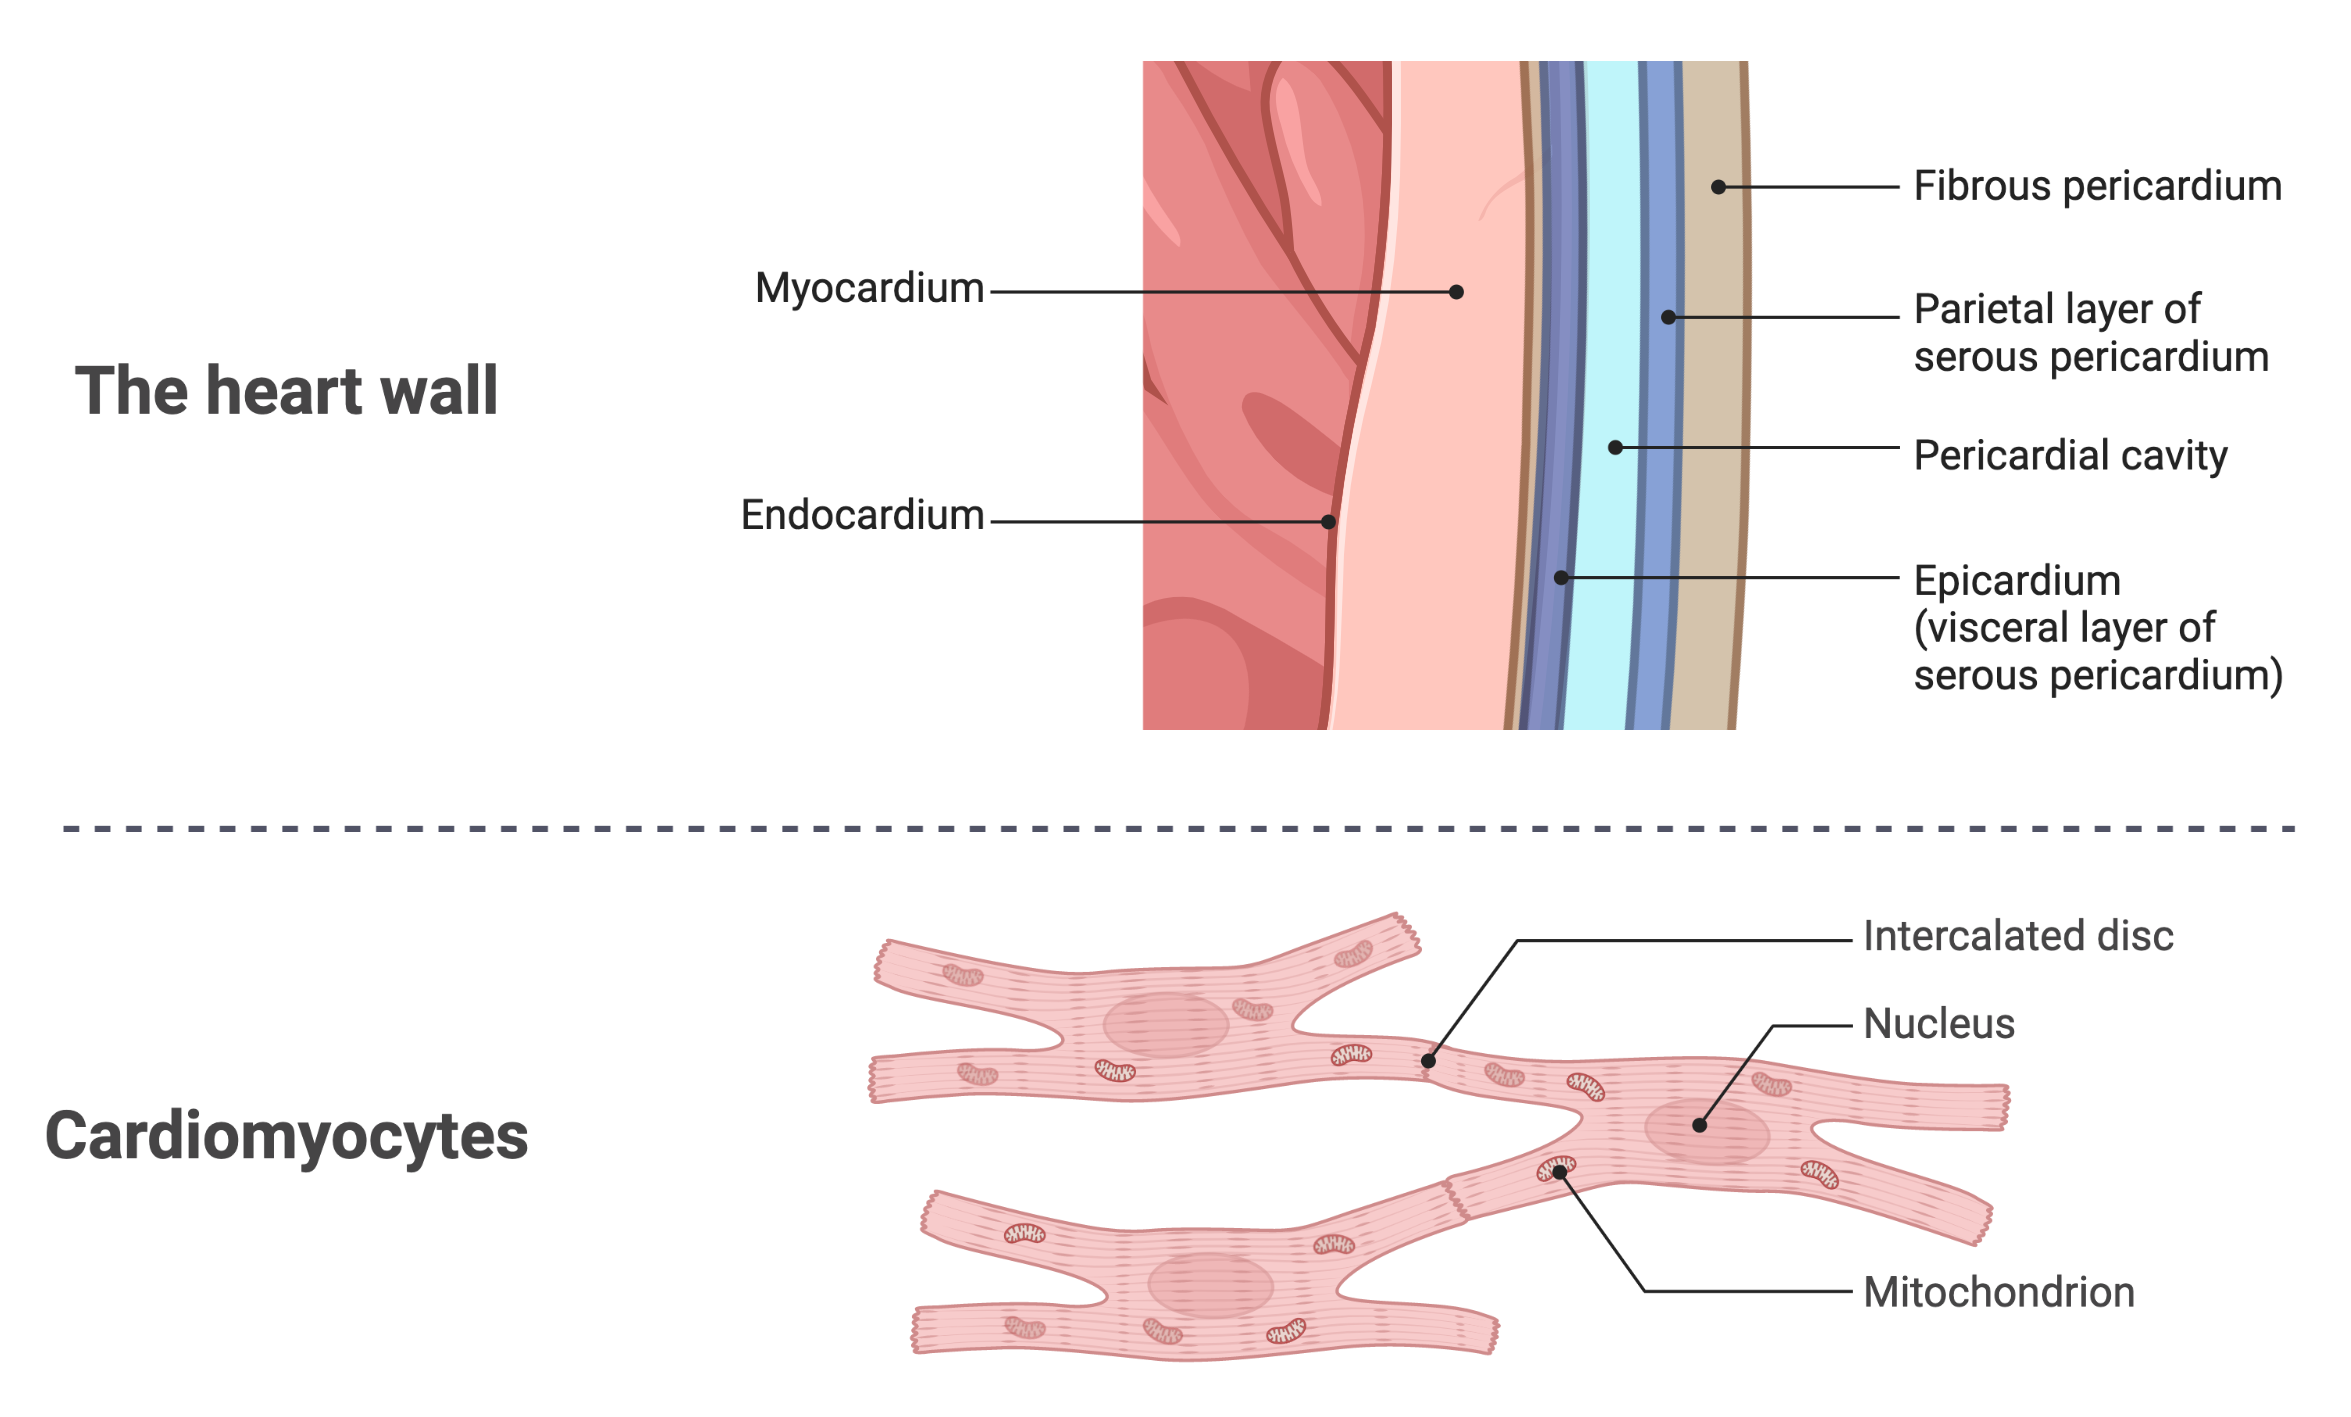
\includegraphics[width=.75\linewidth]{./figure/Cardiac_Muscle.png}
    \caption{Cardiac Muscle \footnotesize{(Created with BioRender.com)}}
    \label{fig:Cardiac_Muscle}
\end{figure}

\paragraph{Volume-Tension Curve}

Cardiac muscle fibers \textit{in vitro} have a length-tension curve that is similar to skeletal muscle fibers. The primary difference is that the passive component is shifted to the left and is a steeper exponential curve. The active component displays a similar curve based on the overlap of actin and myosin. The passive component displays that cardiac muscle has a stiffer form of titin that contributes to tension with a smaller increase in length. 

Cardiac muscle \textit{in situ} has a \textbf{volume-tension curve} that is synonymous with the length-tension curve of whole skeletal muscle. The cardiac volume-tension curve is similar looking to its length-tension curve, the primary difference again being the passive component is shifted further to the left and is steeper. The volume-tension curve is influenced by the length-tension of the cardiac muscles and the passive structures surrounding the heart that resist changes in the chamber size directly. Passive tension starts to develop as the cardiac chamber fills. The functional implication is that under normal resting conditions passive tension contributes to cardiac contraction. And with larger volumes of blood in the chambers the contribution of passive tension rises exponentially.

The passive component of the volume-tension curve is related to cardiac compliance. As described in Chapter \ref{chp:microcirculation} there is a relationship between volume, compliance and pressure. The cardiac muscles vary the volume of chambers while having a particular compliance (that varies with the passive and active tension) for the purpose of generating pressure. This is a fundamental difference between cardiac and skeletal muscle tension. Skeletal muscle tension changes length based directly on tension for the purposes of generating torque. Cardiac muscle tension changes length for the purpose of changing volume and compliance, for the purpose of changing pressure. It is the pressure generated in the cardiac chambers that result in circulation.

Understanding cardiac function requires a familiarity with the equations relating compliance, volume and pressure introduced in Chapter \ref{chp:microcirculation}, repeated here specific for the heart:

\begin{equation}
    \Delta P_{chamber} = \frac{\Delta V_{chamber}}{C_{chamber}}
    \label{eq:Cardiac_Pressure}
\end{equation}

In Equation \ref{eq:Cardiac_Pressure} the dependency of pressure on volume and compliance is clear. Since circulation is a cyclic variation in pressure gradients through the cardiac pump (and vascular vessels), the entirety of cyclic circulation through the heart can be considered from the perspective of cyclic changes to volume and compliance that develop pressure gradients to create flow through and out of the heart. Consideration of volume and compliance for the function of the heart a a pump correctly orients the discussion for both active and passive tension since they both contribute to cardiac pump function.

\subsubsection{Preload}

Preload is the term given for the pressure in a chamber when the cardiac muscle is filled (circulation into the chamber is approaching 0) but is not yet activated. Preload is the passive tension in the chamber right before it develops active tension. Preload for cardiac muscle is analogous to stretch on skeletal muscle. The pressure of preload is related to the volume and the compliance. The compliance is at its highest when the myocardium is empty and not activated. As the chamber fills with blood, passive tension starts to develop which gradually reduces compliance while increasing the volume of blood, which when combined increases pressure. Under normal circumstances this increase in pressure (higher blood volume and lower compliance) is not great enough to fully impede circulation into the chamber. The passive tension developed during preload is subsequently utilized to assist active tension. Which develops the tension necessary to change the volume and compliance of the chamber for the purpose of increasing pressure to facilitate circulation out of the chamber. The increased pressure, alone, simply directs circulation out of the chamber from an area of high to low pressure. The direction of actual circulation through the heart is dependent on properly functioning valves that limit flow "backwards" and allow circulation "forwards" based on cardiac anatomy (Figure \ref{fig:Cardiac_Anatomy}.

The preload is directly related to end-diastolic pressure (EDP), which is directly related to end-diastolic volume (assuming the compliance is normal and relatively low during diastole). The volume that results in preload is from circulation. Where the circulation is coming from for preload depends on the chamber. The right atrium preload comes from the systemic veins; right ventricle preload comes from the right atrium through the tricuspid valve; left atrium preload comes from the pulmonary veins; left ventricle preload comes from the left atrium through the mitral valve. 

It is most common to discuss preload from the perspective of the left ventricle (LV). Therefore, unless otherwise noted, EDV and EDP mean LVEDV and LVEDP (respectively). EDP is related to the \textbf{Frank-Starling law} which states that the amount of venous return influences the performance of the left ventricle (assumes all the venous return moves through the right heart circulation (RA, RV, pulmonary arteries, pulmonary capillaries, pulmonary veins to the LA and finally the LV). The Frank-Starling mechanism is based on the relationship between EDP and total tension developed from active and passive tension.

\subsubsection{Afterload}
Afterload is the term given for the pressure that a chamber must overcome to cause circulation out of the chamber. Afterload for cardiac muscle is analogous with resistance (or load) for skeletal muscle. It is the resistance that the cardiac chamber must exert its tension in order to reduce the volume of the chamber. The pressure of afterload depends on which chamber must overcome that pressure. For the RA it is the pressure exerted on the tricuspid valve by the RV; for the RV it is the pressure exerted on the pulmonic valve by the pulmonary arteries; for the LA it is the pressure exerted on the mitral valve by the LV; for the LV it is the pressure exerted on the aortic valve by the aorta (first of the systemic arteries). 

It is most common to discuss afterload from the perspective of the LV. Therefore, unless otherwise noted, afterload refers to aortic pressure and is best estimated as mean arterial pressure (MAP) (See Equation \ref{eq:MAP_simplified}). MAP is related to vascular compliance and resistance. As afterload, MAP affects aortic valve opening and is the most obvious load encountered by the ejecting ventricle. 

\begin{warning}{HFpEF}
   Long term high blood pressure (hypertension) results in left ventricular hypertrophy (LVH) that is associated with a reduced size and reduced compliance of the LV chamber. LVH is a common cause of diastolic (preserved ejection fraction (pEF)) heart failure (HFpEF).
\end{warning}

\paragraph{Ejection Fraction}

The amount of blood ejected from the LV during systole is called stroke volume (SV). It should be clear that SV is impacted by both preload and afterload. SV is simply the EDV minus the end systolic volume (ESV) ($EDV-ESV$). 

The percentage of blood in the chamber (EDV) that is ejected during systole is the ejection fraction: 

\begin{equation}
    EF = \frac{SV}{EDV}
    \label{eq:LVEF}
\end{equation}

A useful equation to remember for SV is therefore:

\begin{equation}
    SV = EDV \times EF
    \label{eq:SV}
\end{equation}

Equation \ref{eq:SV} highlights how the two phases of the cardiac cycle (systole and diastole) contribute to stroke volume. Diastole contributes with a volume of blood (EDV). Systole contributes the tension to eject a fraction of that blood (LVEF). As discussed above, LVH can cause something called diastolic or preserved EF heart failure (pEF). That is because LVH reduces SV by reducing the size of the LV chamber. It reduces EDV, but does not reduce LVEF. There are also causes of HF that do reduce LVEF and they are called systolic or reduced EF heart failure (rEF). There are also situations - most often due to comorbidities (having more than one condition) - that cause HF with both diastolic (reduced EDV) and systolic (reduced LVEF) components. 

\subsection{Excitation}

To initiate a contraction cardiac muscle must undergo excitation. Excitation of cardiac muscle includes several similarities, but also differences, with skeletal muscle excitation. 

\subsubsection{Automaticity \& Rhythmicity}

Cardiac muscle is self excitatory (automaticity). Self excitations are rhythmic, occurring at rest approximately every 2/3 of a second (650 ms) with very little variability when not influenced by the neuroendocine system (HR of approximately 90 bpm with low heart rate variability (HRV)). Or every 60 seconds with more variability when influenced by the neuroendocrine system at rest (HR of approximately 60 bpm with a HRV of approximately 50-100 ms when measured as a standard deviation with primarily parasympathetic influence).

In normal conditions automaticity occurs in a cluster of myocardial cells in the right atrium known as the \textbf{sino atrial (SA) node} (pacemaker cells). SA node cells have a higher resting permeability to $Na^+$ than axonal or skeletal muscle membranes. Based on this higher permeability to $Na^+$ these cells do not have a sustained (stable) resting membrane potential (See Figure \ref{fig:Cardiac_SA_Node_AP}. As soon as their membrane is repolarized it begins a slow journey back to the threshold potential due to a slow influx of $Na^+$. How long it takes to reach the threshold (pacemaker potential) determines the heart rate. Under normal conditions the SA node cells have the greatest pacemaker potential.

\begin{figure}[!h]
    \centering
    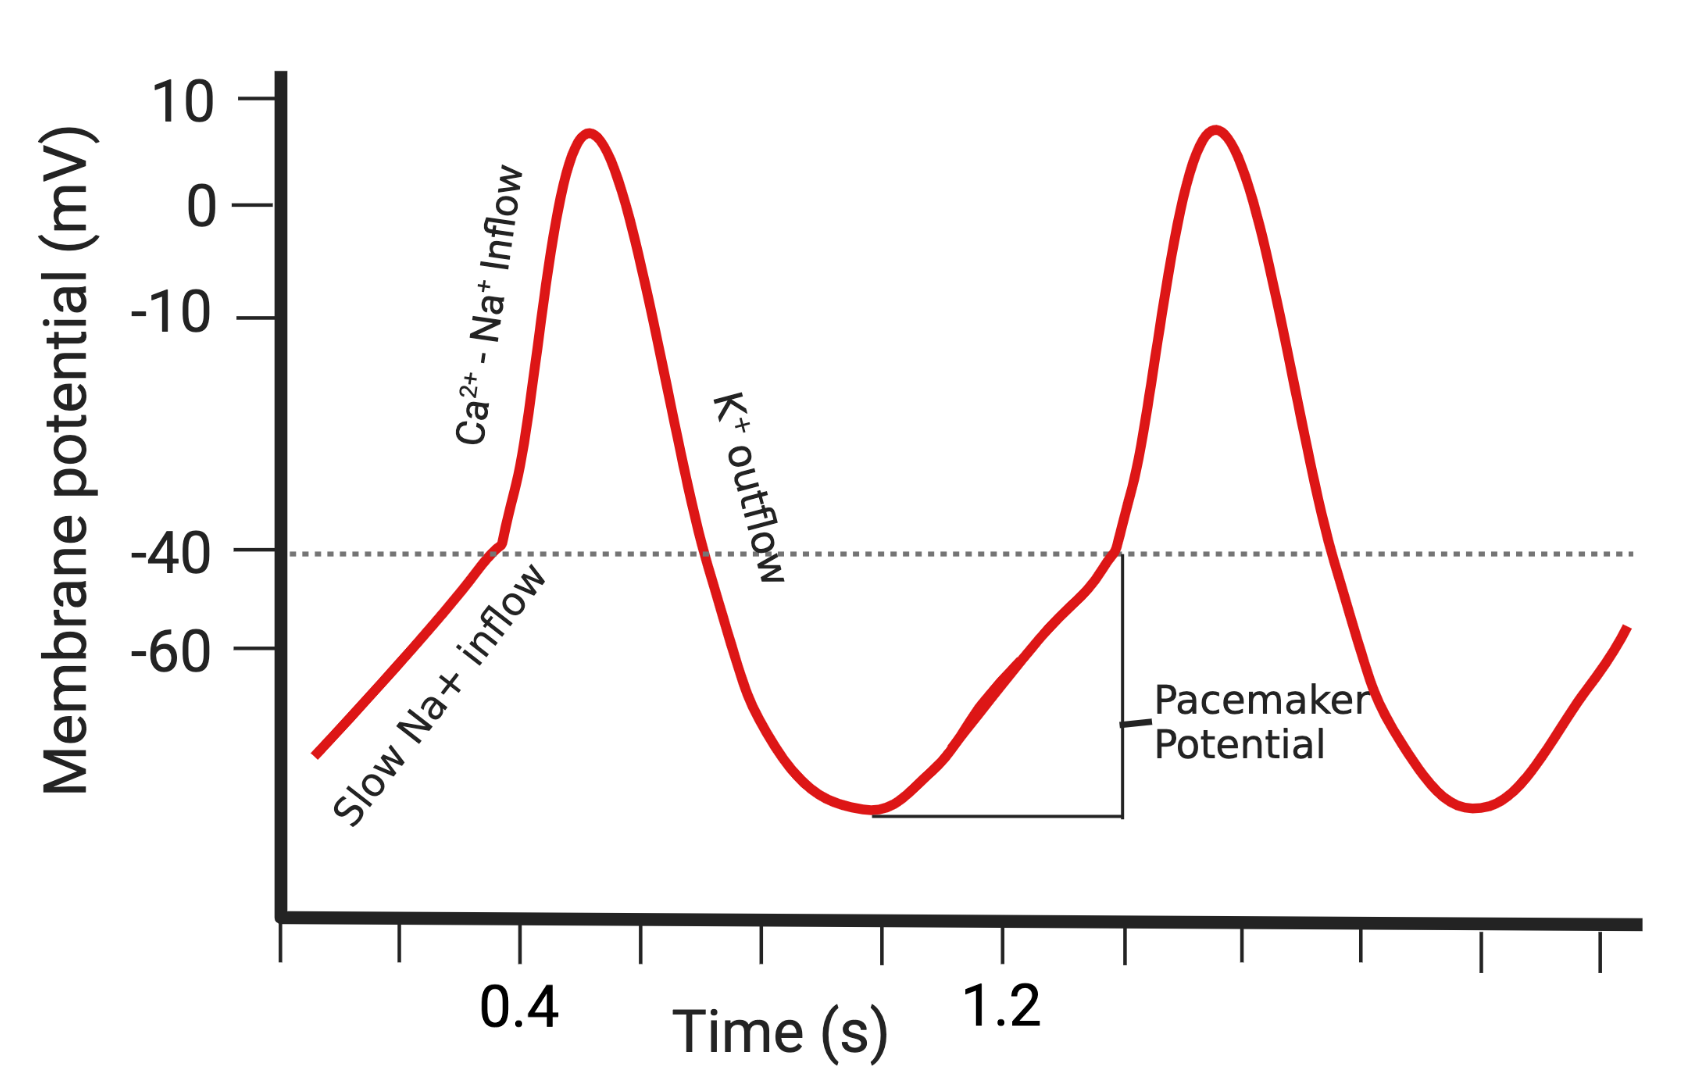
\includegraphics[width=0.5\linewidth]{./figure/Cardiac_SA_Node_AP.png}
    \caption{Cardiac Sino Atrial Node Excitation \footnotesize{(Created with BioRender.com)}}
    \label{fig:Cardiac_SA_Node_AP}
\end{figure}

\subsubsection{Conductivity} 

An excitation of the SA node results in full excitation of all the cardiac muscle cells, first in the atria and after a delay, in the ventricles. There are three features of the myocardium that lead to this pattern of conductivity. 

\begin{figure}[!h]
    \centering
    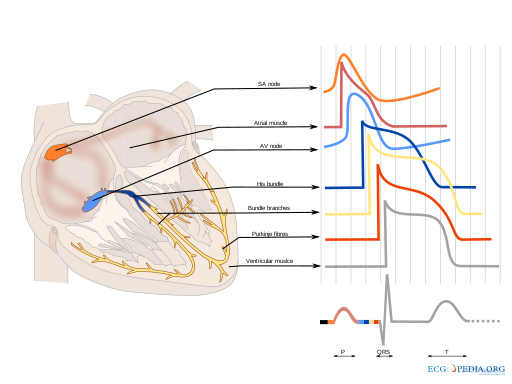
\includegraphics[width=.5\linewidth]{./figure/Cardiac_Conduction.png}
    \caption{Cardiac Conduction \& Shapes of Excitation \footnotesize{(Created with BioRender.com)}}
    \label{fig:Cardiac_Conduction}
\end{figure}

\begin{enumerate}
    \item There are specialized cardiac cells that form a conduction network (See Figure \ref{fig:Cardiac_Conduction}. The conduction network starts with the SA node sending a wave of excitation through the atria, facilitated by intra-nodal fibers (not shown in Figure \ref{fig:Cardiac_Conduction}) that can rapidly carry an excitation from the SA node to the atrio-ventricular (AV) node. The excitation through the atria results in the P wave of the electrocardiograph (ECG). The excitation of the AV node and its distal conduction component, the bundle of His, is slower and delays the excitation of the ventricles (the PR interval on the ECG). Once through the AV node and bundle of His the excitation travels rapidly down the right and left bundle branches to the purkinje fibers. The branching conduction network in the ventricles is critically important to rapid and synchronous excitation of the ventricles (the QRS complex in the ECG). Atrial repolarization is a minor event and is easily lost in the waves of the QRS. Ventricular repolarization is a more substantial event because the ventricles are more substantial muscles and results first in a return to baseline (ST segment on the ECG), and then the T wave on the ECG. It should be noted in Figure \ref{fig:Cardiac_Conduction} that the AV node fibers have a pacemaker potential but it is smaller than the SA node pacemaker potential. The SA node is the pacemaker under normal circumstances because it has a larger pacemaker potential and reaches the excitation threshold earlier than the AV node. However, if the SA node fails, the AV node reaches the excitation threshold and initiates ventricular excitation.
    \item There is a fibrous connective tissue boundary between the atria and the ventricles that does not transmit an excitation (does not have an excitable membrane). This helps ensure that ventricular excitation occurs only through excitation of the AV node (and no other way). The AV node ensures that the ventricular contraction occurs after a delay so that there is time for atrial contraction to push the final 20-30\% of blood into the ventricles for the final stretch of the ventricles which facilitates more tension, thus more pressure for circulation. The "atrial kick" as this is referred facilitates greater tension and thus pressure during ventricular contraction.
    \item Each excitation travels from cardiac muscle fiber to the surrounding cardiac muscle fibers due to the presence of intercalated discs that have gap junctions between cardiac muscle fibers (See Figure \ref{fig:Cardiac_Gap_Junctions}. The presence of these gap junctions not only allows, but greatly expedites, the excitation of one fiber to the next. This is fundamentally different from skeletal muscle where each muscle fiber is insulated from nearby muscle fibers by the endomysium. In skeletal muscle this fiber to fiber excitation would be deleterious to controlled, coordinated movement. But in cardiac muscle the fiber to fiber wave of excitation facilitates a synchronized contraction of all atrial, and then ventricular fibers. Such "all together" contraction facilitates the change in atrial and ventricular chamber size which facilitates the change in pressure necessary for circulation.
\end{enumerate}

\begin{figure}[!h]
    \centering
    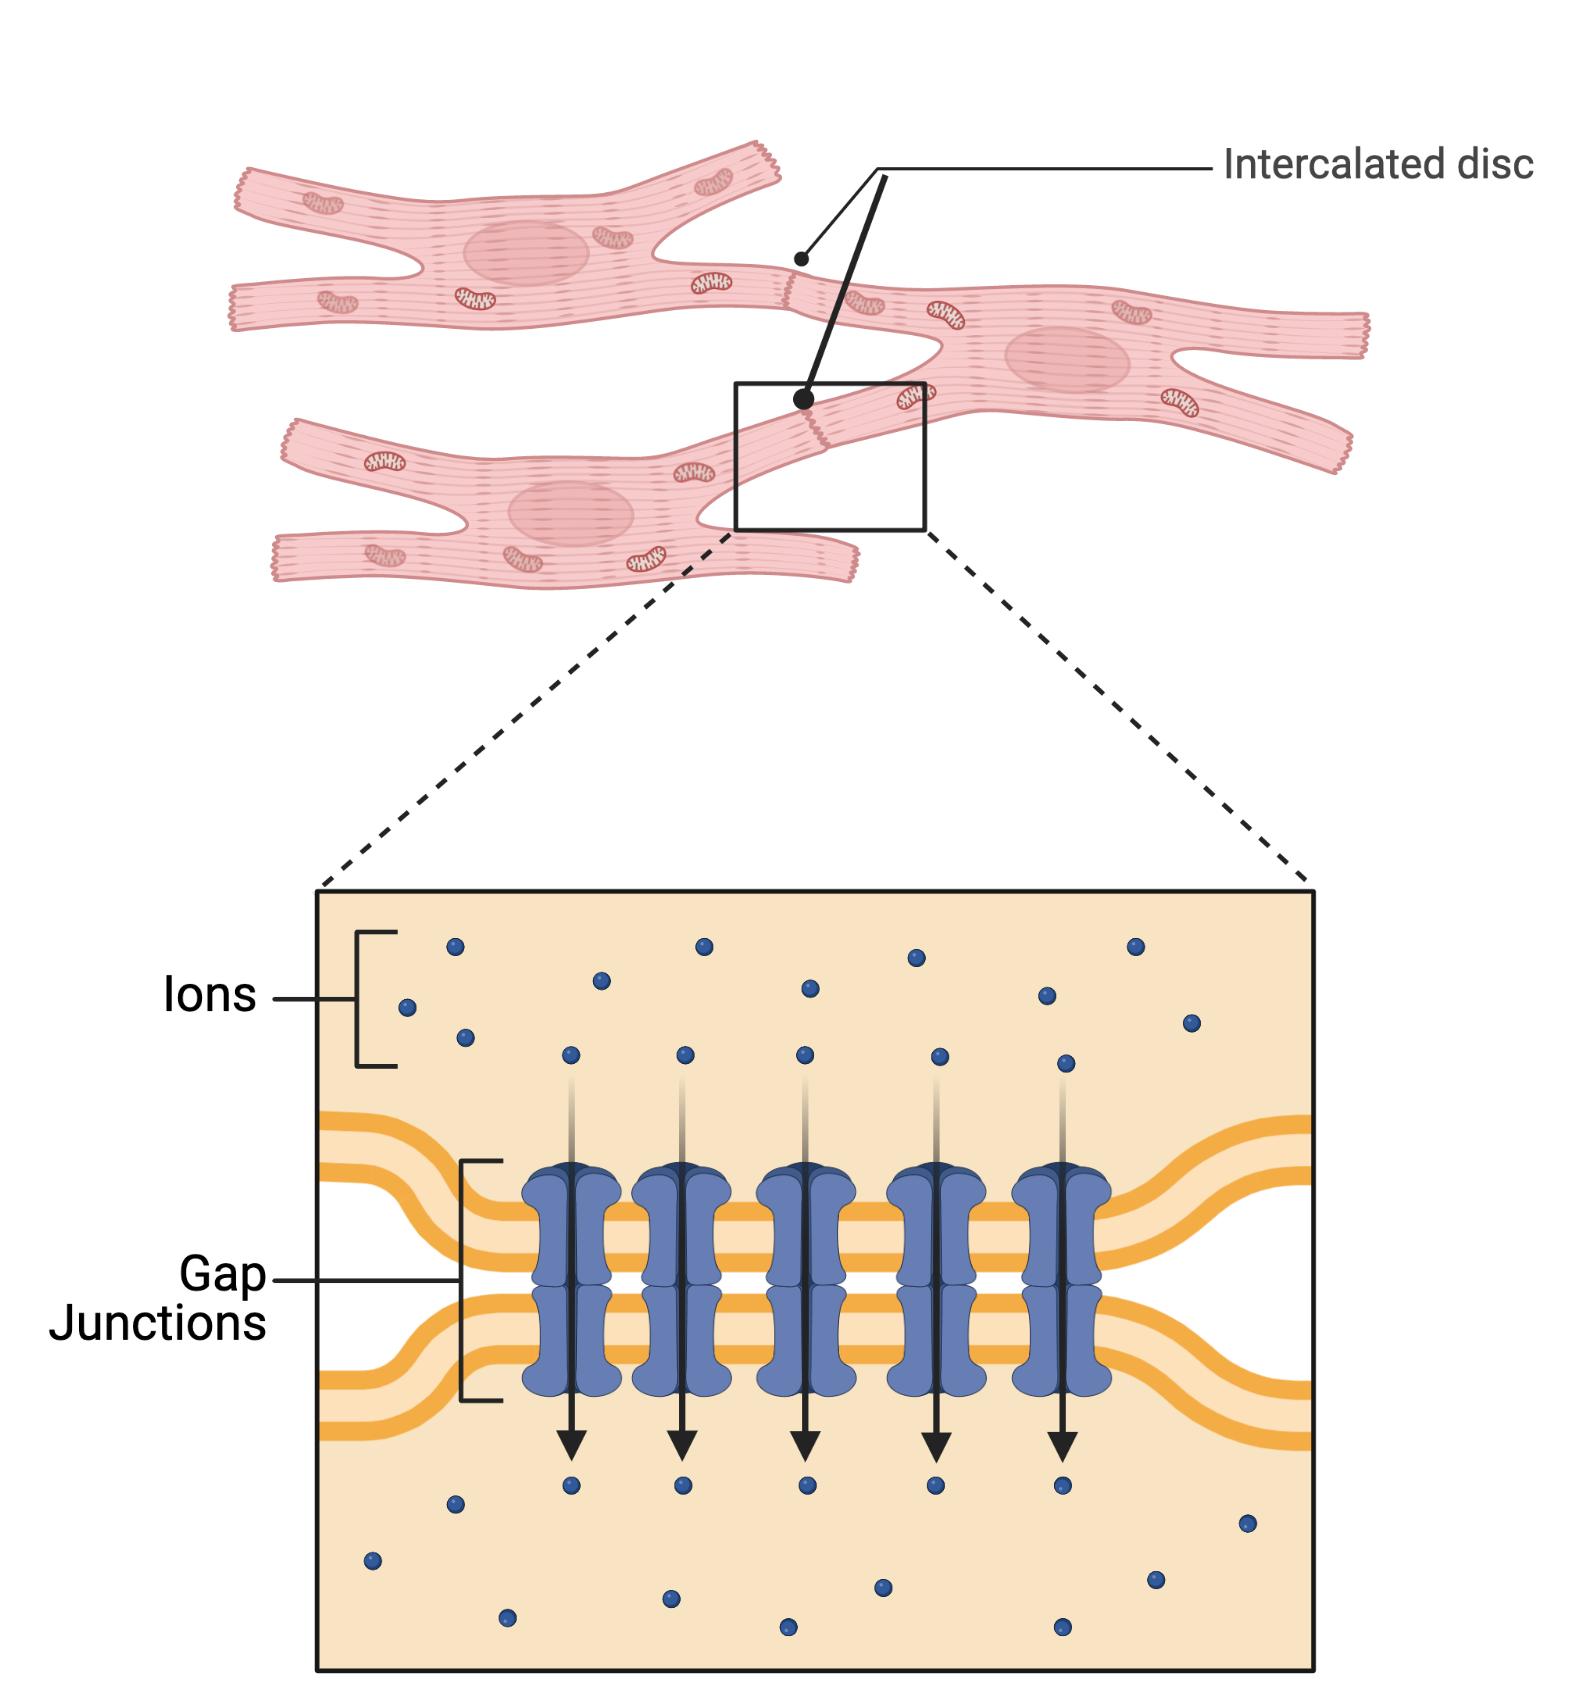
\includegraphics[width=0.5\linewidth]{./figure/Cardiac_Gap_Junctions.png}
    \caption{Intercalated Discs with Gap Junctions \footnotesize{(Created with BioRender.com)}}
    \label{fig:Cardiac_Gap_Junctions}
\end{figure}

\paragraph{Electrocardiogram (ECG)}

The wave of excitation through the cardiac conduction pathway and cardiac muscle fibers generates enough electrical potential to be measured by electrodes on the skin surface. There are several possible electrode placement arrangements, the most popular being referred to as a 12-lead ECG. The 12-lead ECG requires 10 electrodes. Four electrodes are on (or near) the limbs (six limb leads), and six electrodes are on the thorax and surround the heart (six precordial leads). Lead II arises from electrodes on the right arm and left leg and tracks the wave of excitation in the frontal plane from the SA node (origin) through the left ventricle. The ECG wave from Lead II is the most commonly depicted ECG wave. Precordial ECG waveforms that are similar to Lead II include V4, V5 and V6.  Lead II, V4, V5 and V6 are commonly utilized for routine ECG monitoring for arrhythmias. 

A normal ECG is said to display sinus rhythm (sinus referring to the SA node). Figure \ref{fig:ECG} displays the sinus rhythm waves from a normal ECG from a single cardiac cycle from the view of Lead II. Readers are encouraged to view videos of ECG in real time as a preferred approach to becoming familiar with rhythm analysis. A video of normal sinus rhythm is available at this \href{https://youtu.be/Q0JMfIVaDUE?list=PLNN6HI4OXQmyOMNWWrQCCQP559lvbcy4b}{link.} Another option for practicing ECG rhythm analysis is available on iOS and Android devices is the \href{https://simplsim.com/}{Simpl-Simulated Patient Monitor}.

\begin{figure}[!h]
    \centering
    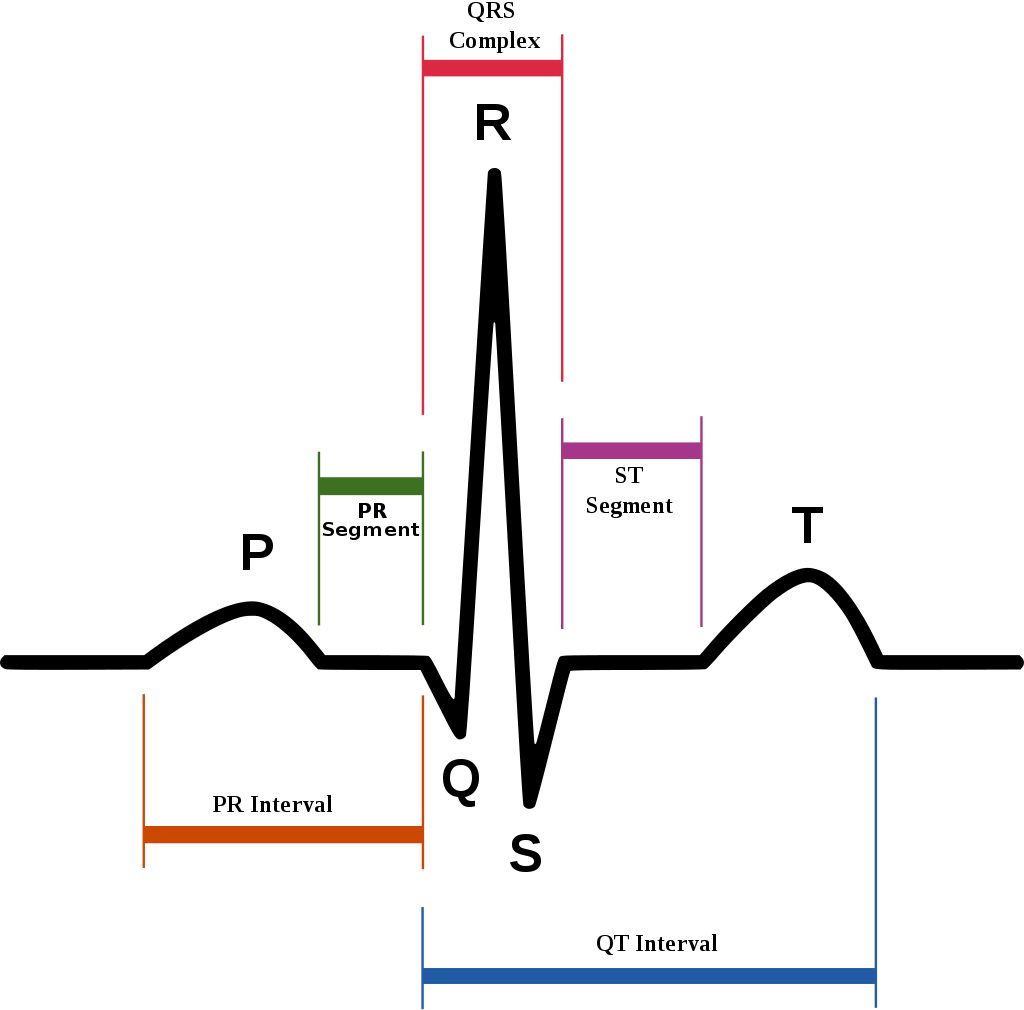
\includegraphics[width=0.5\linewidth]{./figure/ECG.png}
    \caption{ECG Waves (Lead II) \footnotesize{(From Wikipedia  \href{https://commons.wikimedia.org/wiki/File:SinusRhythmLabels.svg}{Sinus Rhythm Labels}, CC BY-SA 4.0)}}
    \label{fig:ECG}
\end{figure}

Table \ref{table:ECGWaves} refers to Figure \ref{fig:ECG} and provides further insight into the excitation event and clinical significance of each wave, segment and interval. ECG abnormalities that must be recognized during real time, single lead rhythm analysis are discussed later in the chapter under practice considerations.

\begin{table}[h!]
\centering
\begin{tabular}{||c c c ||} 
 \hline
 ECG & Excitation Event & Significance \\ [0.5ex] 
 \hline\hline
 P Wave & Atrial Depolarization & SA node, atria \\ 
 PR Segment & AV node delay & AV Node  \\
  PR Interval & SA \& AV node & SA \& AV node  \\
 QRS Complex & Ventricular Depolarization & Ventricles, RR Interval inversely proportional to HR  \\
 ST Segment & Ventricular Repolarization & Ischemia, Injury  \\
 QT Interval & Ventricular De + Repolarization & Long QT syndrome  \\ 
 T Wave & Ventricular Repolarization & Infarction \\ [1ex] 
 \hline
\end{tabular}
\caption{ECG Waves, Segments, Intervals and their excitation events and significance}
\label{table:ECGWaves}
\end{table}


\subsubsection{Contractility}

An excitation results in full tetany of the myocardium and generates enough tension to generate enough pressure for circulation. For a single excitation to result in full contraction of the atria and then the ventricles requires enough $Ca^{2+}$ to be released with one excitation for tetany (not just a twitch). There are two related features that allow for this to occur in cardiac muscle. 

\begin{enumerate}
    \item The cardiac muscle excitation (action potential) is prolonged (See Figure \ref{fig:Cardiac_Ventricular_AP}). It is prolonged due to specialized voltage gated $Ca^{2+}$ channels that allow an inward movement of $Ca^{2+}$ beyond the initiation of the excitation by $Na^+$. The prolonged excitation occurs all the way down to the SR which continues to release $Ca^{2+}$. 
    \item Prolonged SR release of $Ca^{2+}$ into the cell also contributes to the prolonged excitation of the membrane itself (a positive feedback system).
\end{enumerate}

\begin{figure}[!h]
    \centering
    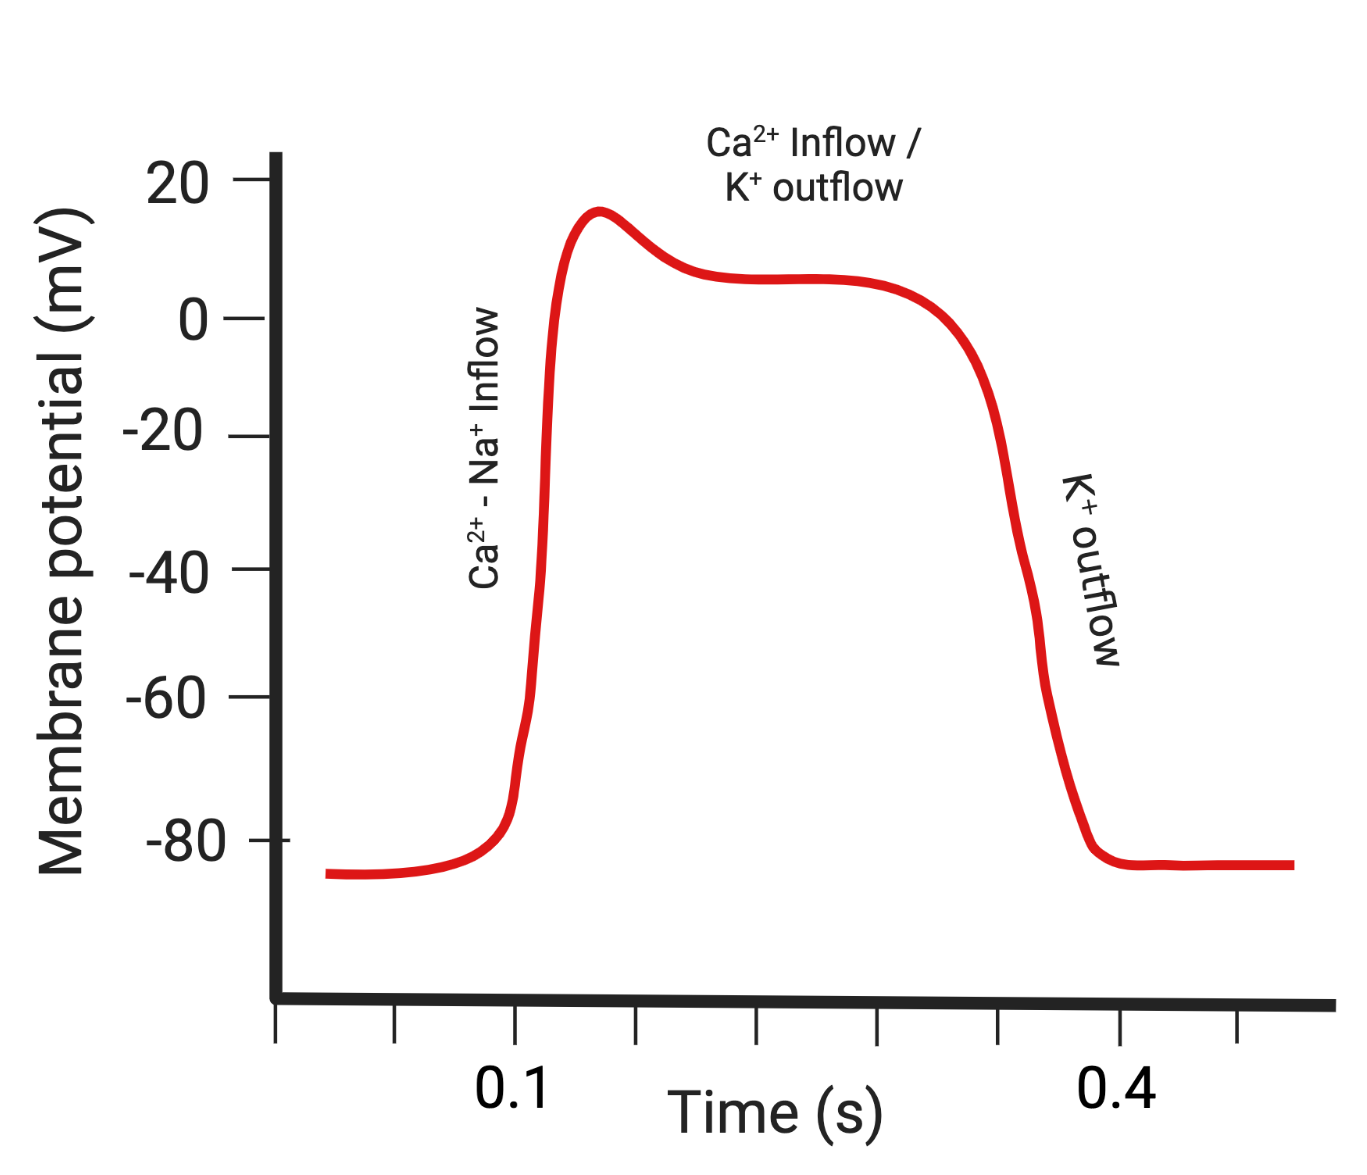
\includegraphics[width=0.5\linewidth]{./figure/Cardiac_Ventricular_AP.png}
    \caption{Ventricular Excitation \footnotesize{(Created with BioRender.com)}}
    \label{fig:Cardiac_Ventricular_AP}
\end{figure}

The primary take away message is that an excitation of a cardiac muscle fiber is prolonged due to inward movement of $Ca^{2+}$ across the sarcolemma, which leads to prolonged SR release of $Ca^{2+}$ for activation that also promotes prolonged excitation. 

\begin{warning}{Cardiac $Ca^{2+}$ Pharmacological Targets}
    Based on the importance of $Ca^{2+}$ in both prolonged excitation and activation of cardiac muscle fibers it is not surprising that medications influencing $Ca^{2+}$ make up two major classes of cardiovascular medications. $Ca^{2+}$-channel blockers decrease the influx from the membrane (anti-arrhythmic) or the SR (anti-hypertensive); and digitalis, which increases the presence of $Ca^{2+}$ in the cardiac muscle fiber.
\end{warning}

\subsection{Regulation}

The regulation of cardiac muscle tension, as part of cardiac pump function (or just cardiac function) is involved in the regulation of $\dot{Q}$. Regulatory mechanisms can vary cardiac pump rate (HR) and vary is contractility (amount of tension and therefore pressure). 

Equations \ref{eq:Q_HRSV} and \ref{eq:SV} are useful models when connecting the regulation of cardiac muscle pump function to $\dot{Q}$. Combining these equations by substituting SV with its components from Equation \ref{eq:SV} results in:

\begin{equation}
    \dot{Q} = HR \times EDV \times LVEF
    \label{eq:Q_HREDVEF}
\end{equation}

\begin{question}{If interested let me know}
    I have a note to myself to make a graphic on the regulation of cardiac function that integrates the past few pages but I don't have the time to do this for this draft. But if anyone does this while studying and is interested in payment for your artwork (if accepted of course), let me know. You'd also get credit for your work in the caption of the figure.
\end{question}

Based on Equation \ref{eq:Q_HREDVEF} there are two ways for cardiac pump function to regulate $\dot{Q}$. As previously discussed the regulation of $\dot{Q}$ results in changes to BP which is regularly monitored to provide feedback.

\begin{enumerate}
    \item Regulate heart rate (HR) - referred to as chronotropy
    \item Regulate tension (contractility) (LVEF) - referred to as inotropy
\end{enumerate}

Equation \ref{eq:Q_HREDVEF} also includes the possibility of using venous return to regulate cardiac pump function. However, venous return is only minimally regulated. Venous return and its EDV are a consequence of venous circulation pressures which are largely determined by skeletal muscle activity. There are changes to vascular tone, but due to the small amount of muscle in the walls of the veins there is much less capacity to regulate venous tone than arterial tone. 

\subsubsection{Neuroendocrine Influence of the Cardiac Pump}

\paragraph{Neural Input}

The autonomic neuroendocrine system influences the heart via direct neural connections and through circulating hormones. It is important to keep in mind that the SA node is the pacemaker. The neuroendocrine input influences, but does not pace, the heart. The multitude of competing external influences to the pacing of HR is one of the reasons for the phenomenon known as HR variability (HRV). 

The parasympathetic (cholinergic) system has direct neural input through the cardiac branch of the vagal nerve (Cranial Nerve X). Vagal nerve activity generally decelerates cardiac function, thus decreasing HR, speed of the conduction wave of excitation and to a lesser extent contractility. The right vagus nerve stimulates primarily the SA node and affects rate, whereas the left vagus nerve stimulates primarily the AV node and affects AV conduction. Note that parasympathetic neural input does not influence EDV. However, EDV can influence parasympathetic neural input (see the Bainbridge reflex below).

Sympathetic (adrenergic) system neural input is through the thoracolumbar sympathetic system and increases HR and augments contractility, thus increasing cardiac function. 

\paragraph{Endocrine Input}
In response to physical activity or stress, the sympathetic nervous system releases catecholamines (epinephrine and norepinephrine) from the adrenal cortex of the adrenal glands which increases HR and contractility. The endocrine influence of the sympathetic nervous system provides a more efficient mechanism for fight/flight signaling since hormones, once circulating in the blood, continue to exert their influence. 

\subsubsection{Cardiac Reflexes}
Cardiac reflexes influence HR and contractility and can be divided into four general categories: baroreflex (pressure) which was discussed in Chapter \ref{chp:circulation}, Bainbridge reflex (stretch), chemoreflex (chemical reflex), ergoreflex (ergoreceptors). 

\paragraph{Bainbridge Reflex}

Mechanoreceptors located in the right atrial myocardium respond to stretch induced by venous return (EDV). An increased volume in the right atrium results in an increased stretch of the atrial wall. This reflex, known as the Bainbridge reflex, stimulates the vasomotor center of the medulla, which, in turn, increases sympathetic input, and decreases parasympathetic input for an overall increased HR and contractility. Respiratory sinus arrhythmia, an increased HR during inspiration and decreased HR during expiration, may be facilitated by changes in venous return and SV caused by changes in thoracic pressure induced by the respiratory cycle. At the beginning of inspiration when thoracic pressure is decreased, venous return and EDV is greater; therefore a greater stretch is exerted on the atrial wall.

\paragraph{Chemoreflexes}
Chemoreceptors located on the carotid and aortic bodies have a primary effect on increasing rate and depth of ventilation in response to $CO_2$ levels, but they also have a cardiac effect. Increased $CO_2$ tends to promote a higher HR and decreased $CO_2$ a lower HR. However, compared to other reflexes and competing influences over HR the chemoreflexes exert a relatively minor influence.

\paragraph{Ergoreflexes}
Ergoreceptors and the ergoreflex regulates circulation through activation of mechanosensitive afferents to inhibit the sustained vagal effects on the heart caused by an increase blood pressure triggering the baroreflex during physical activity that would otherwise work against the overall need for more circulation.


\subsection{Energetics}

Cardiac muscle is exceptionally well developed for aerobic metabolism, even more so than slow oxidative (SO) skeletal muscle fibers. Even during high intensity exercise cardiac muscle is capable of taking in lactate that is circulating in the blood and facilitating its transformation back into pyruvate and acetyl-CoA for entry into the citric acid cycle (TCA). Only when there is a lack of $O_2$ available for electron transport (ETC) do the aerobic energetic pathways not keep up with glycolosis in cardiac muscle cells (there is no normal anaerobic threshold for cardiac muscle). 

Cardiac muscle is so developed for aerobic metabolism that even at rest the myocardium utilizes approximately 80\% of the $O_2$ delivered the blood. Skeletal muscle, at rest, only utilizes approximately 20\% of the $O_2$ that is delivered in the blood. Though much of this difference is based on the difference in resting metabolic need. This makes cardiac muscle critically dependent on increases in circulation to provide the additional $O_2$ needed in response to increased myocardial oxygen demand (RPP).

\begin{warning}{Rate Pressure Product}
    The rate pressure product (RPP), also referred to as the double product, is described by the equation: $RPP = HR \times SBP$, where HR is heart rate and SBP is systolic blood pressure. It is an indication of cardiac muscle (myocardium) oxygen demand. This experimental observation has useful clinical application. It also demonstrates the fact that pressure generated by the myocardium includes active tension which requires oxygen.
    
    In situations with increased afterload the myocardium must develop more pressure for circulation. This greater pressure requires greater tension. This greater tension requires more ATP. More ATP requires more $O_2$. The more frequently the tension is generated (HR) the more ATP and subsequently $O_2$ is required. The experimental association between RPP and myocardial $O_2$ demand is a rather simple consequence of the underlying relationship between pressure (resistance), active tension and ATP.
    
    If a patient undergoes maximal exercise testing and has myocardial ischemia, RPP can be calculated at the point when ischemia is occurring to establish the patient’s ischemic threshold. RPP at the ischemic threshold can then be used during exercise to provide a safe guideline of exercise intensity. This value is useful even if the patient is on a beta-adrenergic antagonist ($\beta$-blocker). Even though the $\beta$-blocker reduces the HR response by blocking the action of epinephrine and norepinephrine on the heart, it is this mechanism that reduces the risk of reaching ischemia. While on a $\beta$-blocker, HR is not a good linear indication of overall aerobic workload (it loses its linear relationship with $\dot{V}O_2$), the RPP is a good discrete indicator of whether a patient is above or below their ischemic threshold. A patient that starts taking a $\beta$-blocker (adrenergic antagonist) will have a harder time exceeding the ischemic threshold, which is the point of being on a $\beta$-blocker for people with ischemic cardiac disease. 
\end{warning}

\begin{comment}

\begin{backgroundinformation}{RPP Example}
    For example: If HR and SBP at rest are 60 beats per minute (bpm) and 110 mmHg then RPP is 6,600. If these values reach 180 bpm and 200 mmHg for an RPP of 36,000 there is a roughly a 5.5 fold increase in myocardial oxygen demand. To meet that demand a roughly 5 fold increase in myocardial circulation (perfusion) must be achieved. This estimate is most accurate if these values are reached at rest (rare). If these values are achieved during exercise they are a small over estimate of the actual myocardial oxygen demand. During exercise there is a significant increase in the skeletal muscle pumping action on venous circulation. Therefore there is a significant increase in venous return. Increased venous return increases preload. Increased preload increases the contribution of passive tension on cardiac contraction. The increased contribution of passive tension on cardiac contraction reduces the myocardial oxygen demand. 
    Therefore, a HR of 180 and SBP of 200 at rest has a higher myocardial oxygen demand than a HR of 180 and SBP of 200 during exercise despite the same RPP because of the contribution of preload and passive tension to cardiac contractility.
\end{backgroundinformation}
\end{comment}

\subsubsection{Cardiac Circulation}

The major coronary arteries include the left coronary (LCA) which quickly branches into the left anterior descending (LAD) and left circumflex (LCx); and the right coronary artery RCA) (See Figure \ref{fig:Cardiac_Circulation}). LAD distributes the anterior wall of both ventricles (L > R) including the septum. LCx the left lateral and posterior walls. LAD and LCx join for distribution in the inferior myocardium. RCA distributes to the anterolateral, lateral, posterior and inferior RV. The RCA and LCA are the first two vessels off of the aorta. Blood is pumped to these large superficial coronary arteries during ventricular systole. At this time, myocardial contraction limits the flow of blood to the myocardium; therefore myocardial tissue is perfused during diastole.

\begin{figure}[!h]
    \centering
    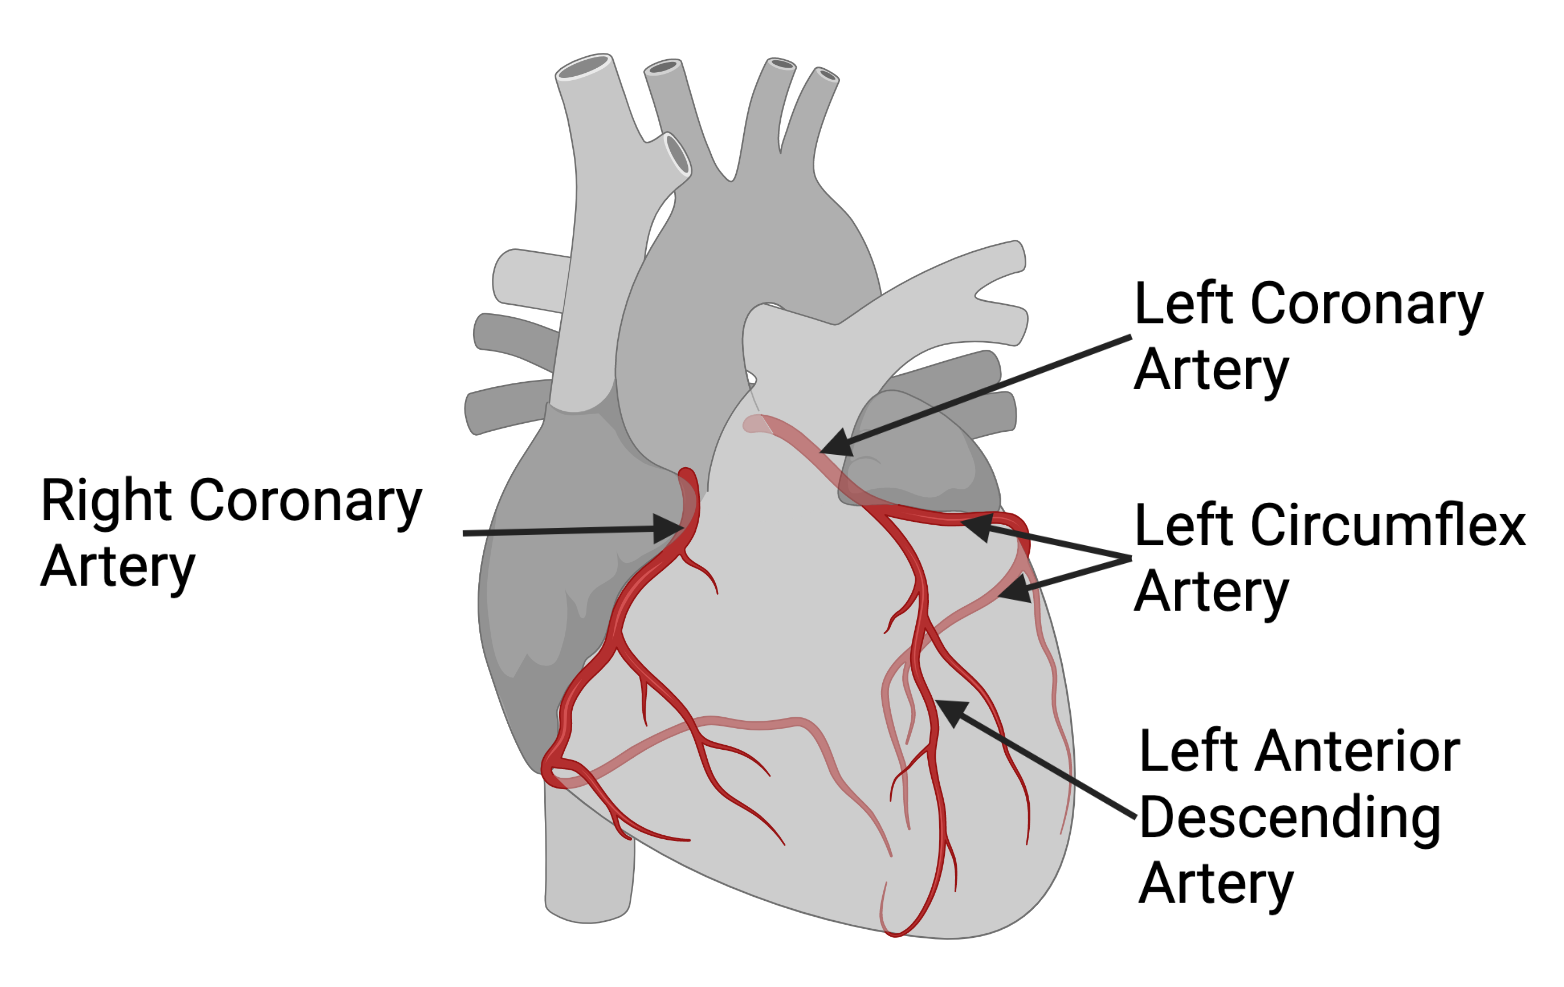
\includegraphics[width=0.5\linewidth]{./figure/Cardiac_Circulation.png}
    \caption{Cardiac Circulation \footnotesize{(Created with BioRender.com)}}
    \label{fig:Cardiac_Circulation}
\end{figure}



\section{Cardiac Cycle}

The events of the cardiac cycle are displayed in Figure \ref{fig:Cardiac_Wiggers}. 
\begin{figure}[!h]
    \centering
    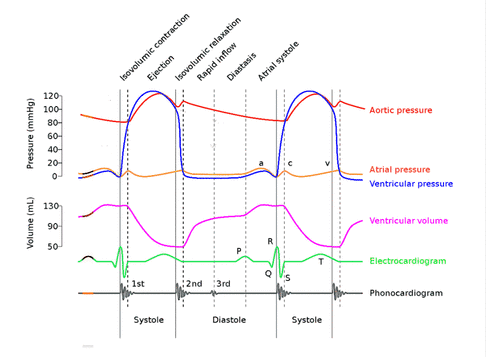
\includegraphics[width=.75\linewidth]{./figure/Cardiac_Wiggers.png}
    \caption{Wiggers Diagram of the Cardiac Cycle \footnotesize{(From Wikipedia  \href{https://en.wikipedia.org/wiki/Wiggers_diagram}{Wiggers Diagram Entry}, CC BY-SA 4.0)}}
    \label{fig:Cardiac_Wiggers}
\end{figure}

Circulation throughout the cardiac cycle depends on circulatory and cardiac pressure gradients. The right side of the heart is a low-pressure system with little vascular resistance in the pulmonary arteries, whereas the left side of the heart is a high-pressure system with high vascular resistance from the systemic circulation. The cardiac cycle is the period from the beginning of one contraction, starting with SA node depolarization, to the beginning of the next contraction. Systole is the period of contraction, and diastole is the period of relaxation. Systole and diastole can also be categorized into atrial and ventricular components.

\begin{itemize}
    \item Atrial diastole is the period of atrial filling. The flow of blood is directed by the higher pressure in the venous circulatory system.
    \item Atrial systole is the period of atrial emptying and contraction. Initial emptying of approximately 70\% of blood occurs as a result of the initial pressure gradient between the atria and the ventricles. Atrial contraction then follows, squeezing out the remaining 30\%. This is commonly referred to as the atrial kick.
    \item Ventricular diastole is the period of ventricular filling. It initially occurs with ease; then, as the ventricle is filled, atrial contraction is necessary to squeeze the remaining blood volume into the ventricle. The amount of stretch placed on the ventricular walls during diastole, referred to as left ventricular end diastolic pressure (LVEDP), influences the force of contraction during systole.
    \item Ventricular systole is the period of ventricular contraction. The initial contraction is isovolumic (i.e., it does not eject blood), which generates the pressure necessary to serve as the catalyst for rapid ejection of ventricular blood. The left ventricular ejection fraction (EF) represents the percent of end diastolic volume ejected during systole and is normally approximately 60\%.
\end{itemize}

\paragraph{Understanding Wiggers Diagram}

Understanding the cyclic events of Wiggers Diagram in Figure \ref{fig:Cardiac_Wiggers} requires an understanding of pressure changes due to volume and volume changes due to pressure. Readers should start from the left and track the changes in each wave, using the ECG as a guide to the excitation events. Once the reader understands each wave they should proceed to observing the coherence between two, then three and finally all of the waves through the two cardiac cycles depicted. An understanding of cardiac function and the cardiac cycle can be confirmed when Figure \ref{fig:Cardiac_Wiggers} can be reproduced based on an understanding of the events (not by memorizing how to reproduce it). Though, some individuals find that learning to reproduce it by memorizing it ultimately leads to an understanding of cardiac function.


\section{ECG Rhythm Analysis}

ECG rhythm analysis allows identification of minor through major cardiac arrhythmias (conduction abnormalities) as well as deviations in wave forms that are associated with ischemia, injury or infarction of the myocardium (myocardial circulation abnormalities). 

Rhythm analysis includes the observation of one ECG lead in real time via a hard wired ECG monitor or a telemetry (wireless) ECG monitor. The first question when observing an ECG is whether it appears normal, that is with all of its waves and segments in order and spaced as expected. A general approach when observing the ECG in real time is to ask:

\begin{itemize}
    \item Is every P wave followed by a QRS?
    \item Is every QRS preceded by a P wave?
    \item Is every QRS followed by a T wave?
    \item Is every T wave preceded by a QRS?
    \item Is every T wave followed by a P wave?
    \item Is every P wave preceded by a T wave?
    \item Is the PR segment normal width?
    \item Is the QRS complex normal width?
    \item Does the ST segment quickly return to baseline?
    \item Are the QRS complexes reasonably and regularly spaced (RR Intervals)?
\end{itemize}


\subsubsection{Arrhythmias}

Examination for arrythmias can occur with any ECG lead (any one of the standard 12, or other less commonly used electrode and lead configurations). Every lead provides the same information about conduction. For example, if a P wave is missing or a PR interval is long in Lead II, it will be equally missing or as long in Lead aVL or V3 (or any of the other leads). 

\paragraph{Tachyarrythmias (Ectopy)}

Tachyarrythmias refer to arrhythmias associated with more excitation than usual during cardiac conduction. Such aberrant excitation usually results in a higher heart rate. Tachycardia is a HR higher than 100 bpm and is not technically an arrhythmia - though if its occurs without provocation (physical, mental or emotional stress) then it may be indicative cardiac or autonomic dysfunction. When tachycardia is unprovoked it is often referred to as supra-ventricular tachycardia (SVT) or atrial tachycardia. The most common type of SVT is paroxysmal SVT (PSVT). Paroxysmal simply means it comes and goes without any currently understood provocation (cause).
There are a group of tachyarrythmias caused by ectopic action potentials that cause ectopic excitations and beats. Ectopic simply means these excitations are not originating in the SA node and following the normal excitation conduction pathway. Ectopy originates from an ectopic focus (myocardial cells causing an action potential) or if more than one focus, as ectopic foci. An ectopic focus (or foci) can occur due to myocardial cell irritation (producing an excitation when it should not, i.e. caffeine or other stimulants), or due to myocardial cell depression (delay or block in conduction caused by ischemia, injury or scar tissue) that produces a recurrent loop of self perpetuating excitation within the myocardium). 

Table \ref{table:Tachyarrhythmias} organizes six different tachyarrhythmias based on where they occur (atria or ventricles) and the regularity of the ectopic focus (or foci) excitations.

\begin{table}[h!]
\centering
\begin{tabular}{||c c c ||} 
 \hline
   & Atria & Ventricle \\ [0.5ex] 
 \hline\hline
 Occasional Ectopic Focus & Premature Atrial Contr. (PACs) & Premature Ventricular Contr. (PVCs)\footnotemark\footnotetext{Also referred to generally as ventricular ectopy or ventricular premature beats (VPBs)} \\ 
 Occasional Ectopic Foci & PACs & Multifocal PVCs \\
 Non Stop Ectopic Focus & Atrial Flutter (AFlutter)& Ventricular Tachycardia (VTach)  \\
 Non Stop Ectopic Foci & Atrial Fibrillation (AFib) & Ventricular Fibrillation (VFib)  \\ [1ex] 
 \hline
\end{tabular}
\caption{Types of Ectopic Tachyarrhythmia}
\label{table:Tachyarrhythmias}
\end{table}

The severity of all conduction abnormalities is based on the impact they have on cardiac output and blood pressure (hemodynamics). In general the impact a tachyarrhythmia has on hemodynamics is greater proceeding down the rows; and is always greater in the ventricular column than the atrial column. For example, PACs have little, if any, impact on hemodynamics; whereas VFib does not produce any circulation at all so there is no cardiac output and no blood pressure (and therefore no pulse). 

Since the tachyarrhytmias exist on a spectrum, it is required that a physical therapist can identify which tachyarrhytmia is present should one arise (or be part of a patient's chronic condition). For example, it is not appropriate to stop activity due to AFib in a patient with chronic AFib, but it is important to monitor the ventricular rate and BP for signs of worsening hemodynamics in AFib. Nor is it required to stop activity due to PACs or PVCs in all situations. 

A YouTube playlist of tachyarrhythmias is available at this \href{https://www.youtube.com/playlist?list=PLNN6HI4OXQmwFdE8LVIGC_l5WG2ViWAy3}{link.}

\paragraph{Bradyarrythmias \& Blocks}

Bradycardia refers to any HR below 50 bpm. However, like tachycardia, bradycardia does not always indicate there is a conduction problem. Whether bradycardia is a problem comes down to whether it is creating problems with hemodynamics. Generally, if there is an abnormality causing bradycardia it will provoke problematic changes in hemodynamics, for example, sick sinus syndrome or third degree AV block. A normal cause of bradycardia that does not provoke problematic changes in hemodynamics is being well conditioning from exercise training.

Bradyarrhythmias can be caused by AV blocks, though not all instances of AV blocks create bradycardia. It is just common to classify blocks as a bradyarrhythmia. There are three degrees of AV Block, and four types (there are two types of second degree AV block).

\begin{itemize}
    \item First Degree AV Block: Prolonged PR Interval
    \item Second Degree AV Block - Mobitz 1 (Wenkebach) - progressive prolongation of the PR interval until finally there is a P wave without a QRS indicating the conduction was blocked which is then followed by a normal PR interval that begins progressive prolongation (this pattern repeats)
    \item Second Degree AV Block - Mobitz 2 - normal PR interval with an occasional P wave with no QRS
    \item Third Degree AV Block - complete AV block (also referred to as complete heart block) P waves and aberrant looking QRS complexes are completely dissociated (though may occasionally align so identification requires watching the ECG for several cycles)
\end{itemize}

A YouTube playlist of bradyarrhythmias and AV blocks is available at this \href{https://www.youtube.com/playlist?list=PLNN6HI4OXQmyt5Ql2um3MthEtLkdJnywd}{link.}

The severity of AV blocks is related to the impact they have hemodynamics. As can be expected, the severity increases from First Degree to Third Degree. Mobitz 2 is considered more severe to Mobitz 1, not due to hemodynamic differences, but because it is more likely to deteriorate into Third Degree AV block.

\subsection{Myocardial Circulation Abnormalities}

Abnormalities in myocardial circulation (perfusion) such as ischemia lead to hypoxic conditions in the myocardial cells. If the ischemia persists cell death will occur. Prior to cell death an early indication of ischemia includes changes to the ST segment of the ECG. In a very general way, ST changes are indicative of ischemia and/or injury. This more general fact is sometimes made more specific, with ST depression taken as a sign of myocardial ischemia and ST elevation taken as a sign of myocardial injury. Myocardium that is injured may be reversibly injured (will recover) or irreversibly injured (will die, infarction). 

A YouTube playlist of ST segment changes is available at this \href{https://www.youtube.com/playlist?list=PLNN6HI4OXQmyHL-CDiLqrBSkv6E1Vk0cS}{link.}

One of the problems with the more specific claims of ST changes is that it assumes the ECG lead being observed is a lead that has the best view of the myocardium that has ischemia. Unlike the the arrhythmias which are seen equally well in all ECG leads, a circulation abnormality resulting in ischemia is local to the region of the myocardium with the circulation abnormality (rarely the entire myocardium). For example, aVR tends to have a reversed polarity to Lead II (what goes up in Lead II, goes down in aVR; what goes down in Lead II, goes up in aVR). If ischemia is in an area that Lead II shows depression, it may appear as elevation in aVR. During the diagnostic process (a cardiac stress test) a 12 lead ECG is utilized and additional testing strategies are utilized to confirm that what was observed was in fact ischemia. A cardiologist can get a good idea of where the ischemia is occurring from the 12-lead ECG, which is then confirmed with imaging (nuclear scans or catheterization). When it is known which location (and therefore lead) best pin points the area with a propensity for ischemia then that lead (or a couple of leads) can be utilized for rhythm monitoring. In such situations it is mostly true that ischemia appears as ST depression, and injury appears as ST elevation.

Since the physical therapist using rhythm analysis is primarily interested in identifying abnormalities that warrant the cessation of activity and alerting members of the medical team of such abnormalities (not in making a diagnosis), simply identifying ST changes is sufficient. Both ischemia and injury are sufficient reason to stop activity and alert members of the medical team. In fact, the risk associated with myocardial ischemia and injury is sufficient to warrant extra caution and stopping activity if ST changes are suspected while observing the ECG rhythm. In other words, if the ST segment appears above or below the baseline its safer to assume it is than to assume it isn't. Cease activity and continue monitoring. As with any such signs, noting other signs and symptoms is warranted (shortness of breath, diaphoresis, chest pain, blood pressure, respiratory rate).

\section{Summary}

The cardiac pump supports circulation. Cardiac muscle includes several characteristics required for its unique role in circulation. Cardiac muscle tension, excitation and regulation support circulation and pressure regulation. Excitation of cardiac muscle can be recorded with the ECG and offers insights into several abnormalities of conduction as well as myocardial ischemia. Monitoring the ECG provide physical therapists with non-invasive insights, that when combined with an understanding of circulatory physiology, provide useful information when working with clients both with and without conditions that directly affect the circulation.

\subsection{Next Step}

With an understanding of mass balance and circulation we can now proceed to the mass balance of oxygen and carbon dioxide in the next two chapters. First we consider Respiration which focuses on gas exchange between the alveoli and blood. Then we turn to Ventilation which focuses on air exchange between the environment and the alveoli (breathing).

\printbibliography[heading=subbibintoc]

\section*{Sample Questions}

\begin{enumerate}
    \item Normal end diastolic volume (EDV) is directly related to normal end diastolic pressure (EDP) and normal ventricular compliance. If a pathology results in reduced ventricular compliance during diastole what would occur?
    \item What myocardium features lead to the normal pattern of myocardial conductivity?
    \item Why is cardiac muscle excitation (action potential) prolonged and what changes to the action potential allow this to occur?
    \item How are options for determining and monitoring ischemic threshold during exercise? 
    \item Which cardiac arrhythmia results in an irregularly irregular pulse rhythm?
\end{enumerate} 